\section{Introduction}

In Section \ref{sec:input_space_partitioning} we were able to characterise the input space partitioning induced by a deep network. However, an analytic closed-form formula for the regions alluded us. In this chapter we aim to rectify that by using power diagrams. 

\section{Power Diagrams}

\begin{definition}
    A power diagram partitions a space $\mathcal{X}$ into $r$ disjoint regions $\Omega=\{\omega_1,\dots,\omega_r\}$ such that $\bigcup_{j=1}^r\omega_j=\mathcal{X}$, with $$\omega_j=\{\mathbf{x}\in\mathcal{X}:\nu(\mathbf{x})=j\}$$for $j=1,\dots,r$ where $\nu(\mathbf{x})=\argmin_{i=1,\dots,r}\left(\left\Vert\mathbf{x}-[\mu]_{i,\cdot}\right\Vert^2-[\tau]_i\right)$, for centroids $[\mu]_{i,\cdot}$ and radius $[\tau]_i$.
\end{definition}

Observe how a power diagram is invariant under global shifting of the radii, $$\argmin_{i=1,\dots,r}\left(\left\Vert\mathbf{x}-[\mu]_{i,\cdot}\right\Vert^2-[\tau]_{i,\cdot}\right)=\argmin_{i=1,\dots,r}\left(\left\Vert\mathbf{x}-[\mu]_{i,\cdot}\right\Vert^2-\left([\tau]_{i,\cdot}+q\right)\right).$$

\section{Max-Affine Splines}

A max-affine spline operator with $k$ output dimensions and input space $\mathcal{X}$, is constituted from $k$ max-affine spline units, with the $i^{\text{th}}$ having the computation 
\begin{equation}\label{eq:maso_unit_operation}
    [\mathbf{z}(\mathbf{x})]_i=\max_{j=1,\dots,r}\left\langle[A]_{i,j,\cdot},\mathbf{x}\right\rangle+[B]_{i,j}=\max_{j=1,\dots,r}\mathcal{E}_{i,j}(\mathbf{x}),
\end{equation}
where $\mathcal{E}_{i,j}(\mathbf{x})$ is the projection of $\mathbf{x}$ onto the hyperplane parameterized by $[A]_{i,j,\cdot}$ and $[B]_{i,j}$.

Let $$\mathcal{E}^+_{i,j}=\left\{(\mathbf{x},y)\in\mathcal{X}\times\mathbb{R}:y\geq\mathcal{E}_{i,j}(\mathbf{x})\right\}.$$

\begin{proposition}\label{prop:image_mas_input_space}
    The $i^\text{th}$ max-affine unit maps its input space onto the boundary of the convex polytope $\mathcal{P}_i=\bigcap_{j=1}^{r}\mathcal{E}_{i,j}^+$, leading to $$\mathcal{X}\times[\mathbf{z}]_i(\mathcal{X})=\partial\mathcal{P}_i,$$where $$[\mathbf{z}]_i(\mathcal{X})=\mathrm{Im}\left([\mathbf{z}]_i\right)=\left\{[\mathbf{z}(\mathbf{x})]_i:\mathbf{x}\in\mathcal{X}\right\}.$$
\end{proposition}

\begin{tproof}
    $(\subseteq)$\\Let $(\mathbf{x},y)\in\mathcal{X}\times[\mathbf{z}]_i(\mathcal{X})$. Then $y=\mathcal{E}_{i,j^\prime}(\mathbf{x})$ for some $j^\prime\in\{1,\dots,r\}$ and $y\geq\mathcal{E}_{i,j}(\mathbf{x})$ for every $j=1,\dots,r$. Therefore,
    \begin{align*}
        (\mathbf{x},y)&\in\mathcal{P}_i\setminus\mathrm{int}\left(\mathcal{P}_i\right)\\&=\overline{\mathcal{P}_i}\setminus\mathrm{int}\left(\mathcal{P}_i\right)\\&\subseteq\partial\mathcal{P}_i.
    \end{align*}
    $(\supseteq)$\\We proceed by induction on $r$. 
    \begin{itemize}
        \item For $r=1$ we have
        \begin{align*}
            \partial\mathcal{P}_i&=\partial\mathcal{E}_{i,1}^+\\&=\left\{(\mathbf{x},y):y=\mathcal{E}_{i,1}(\mathbf{x})\right\}\\&\subseteq\mathcal{X}\times[\mathbf{z}]_i(\mathcal{X}).
        \end{align*}
        \item Assume that $$\mathcal{X}\times[\mathbf{z}]_i(\mathcal{X})\subseteq\partial\mathcal{P}_i=\partial\left(\bigcap_{j=1}^{n-1}\mathcal{E}_{i,j}^+\right).$$
        \item For $r=n$ we have
        \begin{align*}
            \partial\mathcal{P}_i&=\partial\left(\bigcap_{j=1}^{n-1}\mathcal{E}_{i,j}^+\cap\mathcal{E}_{i,j}^+\right)\\&\subseteq\left(\overline{\bigcap_{j=1}^{n-1}\mathcal{E}_{i,j}^+}\cap\partial\mathcal{E}_{i,n}^+\right)\cup\left(\partial\left(\bigcap_{j=1}^{n-1}\mathcal{E}_{i,j}^+\right)\cap\overline{\mathcal{E}_{i,n}^+}\right)\\&=\left(\bigcap_{j=1}^{n-1}\mathcal{E}_{i,j}^+\cap\left\{(\mathbf{x},y):\mathcal{E}^+_{i,n}=y\right\}\right)\\&\quad\cup\left(\partial\left(\bigcap_{j=1}^{n-1}\mathcal{E}_{i,j}^+\right)\cap\mathcal{E}_{i,n}^+\right)\\&\subseteq\mathcal{X}\times[\mathbf{z}]_i(\mathcal{X}).
        \end{align*}
    \end{itemize}
\end{tproof}

\begin{figure}
    \centering
    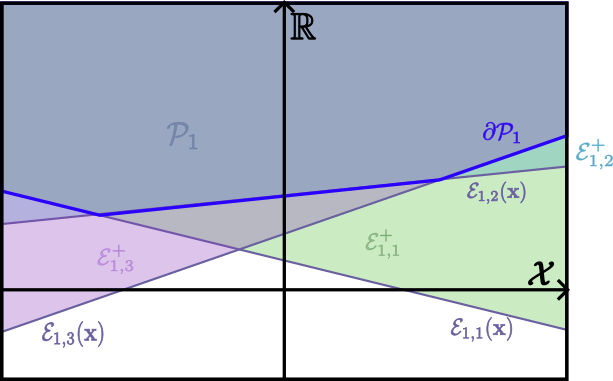
\includegraphics[width=0.75\linewidth]{drawings/max_affine_unit_partition.png}
    \caption{}
    \label{fig:max_affine_unit_partition}
\end{figure}

\begin{lemma}\label{maso_unit_pd}
    The vertical projection on the input space $\mathcal{X}$ of the faces of $\mathcal{P}_i$ from Proposition \ref{prop:image_mas_input_space} construct regions of a power diagram through $$\nu_i(\mathbf{x})=\mathrm{argmax}_{j=1,\dots,r}\mathcal{E}_{i,j}(\mathbf{x}).$$
\end{lemma}

\begin{tproof}
    The faces of $\mathcal{P}_i$ constitute the boundary $\partial\mathcal{P}_i$, which from Proposition \ref{prop:image_mas_input_space} are points $(\mathbf{x},y)$ where $y\geq\mathcal{E}_{i,j}(\mathbf{x})$ for every $j\in\{1,\dots,r\}$ and $y=\mathcal{E}_{i,j^\prime}(\mathbf{x})$ for $j^\prime\in\mathcal{J}\subseteq\{1,\dots,r\}$, where $\mathcal{J}\neq\emptyset$. When $\mathcal{J}=\left\{j^\prime\right\}$, the point $(\mathbf{x},y)$ is an interior point to a face and is vertically projected, through \eqref{eq:maso_unit_operation}, to an interior point of $$\omega_{j^\prime}:=\left\{\mathbf{x}\in\mathcal{X}:\argmax_{j=1,\dots,r}\mathcal{E}_{i,j}(\mathbf{x})=j^\prime\right\}.$$Clearly, the sets $\left\{\omega_1,\dots,\omega_r\right\}$ have disjoint interior, with boundaries between them corresponding to boundaries between faces. Moreover, the set $\left\{\omega_1,\dots,\omega_r\right\}$ cover $\mathcal{X}$ and thus form a power diagram.
\end{tproof}

\begin{theorem}
    The $i^\text{th}$ max-affine unit partitions its input space according to a power diagram with $r$ centroids given by $[\mu]_{i,j}=[A]_{i,j}$ and $[\tau]_{i,j}=2[B]_{i,j}+\left\Vert[A]_{i,j,\cdot}\right\Vert^2$ for all $j\in\{1,\dots,r\}$.
\end{theorem}

\begin{tproof}
    Observe that
    \begin{align*}
        \argmax_{j=1,\dots,r}\left(\mathcal{E}_{i,j}(\mathbf{x})\right)&=\argmax_{j=1,\dots,r}\left(\left\langle[A]_{i,j,\cdot},\mathbf{x}\right\rangle+[B]_{i,j}\right)\\&=\argmax_{j=1,\dots,r}\left(2\left\langle[A]_{i,j,\cdot},\mathbf{x}\right\rangle+2[B]_{i,j}\right)\\&=\argmax_{j=1,\dots,r}\left(\left\Vert[A]_{i,j,\cdot}\right\Vert^2-\left\Vert[A]_{i,j,\cdot}\right\Vert^2+2\left\langle[A]_{i,j,\cdot},\mathbf{x}\right\rangle+\left\Vert\mathbf{x}\right\Vert^2+2[B]_{i,j}\right)\\&=\argmax_{j=1,\dots,r}\left(-\left\Vert[A]_{i,j,\cdot}-\mathbf{x}\right\Vert^2+\left\Vert[A]_{i,j,\cdot}\right\Vert^2+2[B]_{i,j}\right)\\&=\argmin_{j=1,\dots,r}\left(\left\Vert[A]_{i,j,\cdot}-\mathbf{x}\right\Vert^2-\left(\left\Vert[A]_{i,j,\cdot}\right\Vert^2+2[B]_{i,j}\right)\right).
    \end{align*}
    Therefore, we conclude using Lemma \ref{lem:maso_projection_polytope}.
\end{tproof}

\begin{corollary}
    The input space partitioning of a deep network unit is composed of convex polytopes.
\end{corollary}

\section{Max-Affine Spline Operator}

A max-affine spline operator is made by concatenating $k$ max-affine spline units. Let $$\boldsymbol{\nu}(\mathbf{x})=\left(\nu_1(\mathbf{x}),\dots,\nu_k(\mathbf{x})\right)$$and$$E^+_{\boldsymbol{\nu}}=\left\{(\mathbf{x},\mathbf{y})\in\mathcal{X}\times\mathbb{R}^k:[\mathbf{y}]_1\geq\mathcal{E}_{1,\nu_1}(\mathbf{x}),\dots,[\mathbf{y}]_k\geq\mathcal{E}_{1,\nu_k}(\mathbf{x})\right\}.$$

\begin{proposition}\label{prop:image_maso_input_space}
    The layer operator $\mathbf{z}$ maps its input space into the boundary of the $\dim(\mathcal{X})+k$ dimensional convex polytope $\mathbf{P}=\bigcap_{\boldsymbol{\nu}\in\{1,\dots,r\}^k}E_{\boldsymbol{\nu}}^+$ as $$\mathcal{X}\times\mathbf{z}(\mathcal{X})=\mathcal{X}\times [\mathbf{z}]_1(\mathcal{X})\times\dots\times[\mathbf{z}]_k(\mathcal{X})=\partial\mathbf{P}.$$
\end{proposition}

\begin{lemma}\label{lem:maso_projection_polytope}
    The vertical projection on the input space $\mathcal{X}$ of the faces of the polytope of $\mathbf{P}$ from Proposition \ref{prop:image_maso_input_space} construct regions of a power diagram through $\boldsymbol{\nu}$.
\end{lemma}

\begin{theorem}\label{thm:maso_power_diagram}
    A deep network layer partitions its input space according to a power diagram with $\{1,\dots,r\}^k$ cells, centroids $\mu_{\boldsymbol{\nu}}=\sum_{j=1}^k[A]_{j,\nu_j,\cdot}$ and radii $\tau_{\boldsymbol{\nu}}=2\left\langle\mathbf{1},B_{\boldsymbol{\nu}}\right\rangle+\left\Vert\mu_{\boldsymbol{\nu}}\right\Vert^2$.
\end{theorem}

\begin{corollary}
    The input space partitioning of a deep network layer is composed of convex polytopes.
\end{corollary}

\section{Deep Network}

The power diagram partitioning of an $L$-layer deep network can be constructed recursively; each per layer polytope subdivides the previous layer's partitioning.

\newthought{Initialization} identifies the part of the input space of interest $\mathcal{X}^{(0)}\subseteq\mathbb{R}^d$.

\newthought{Layer one} recursion subdivides $\mathcal{X}^{(0)}\subseteq\mathbb{R}^d$ into a power diagram from Theorem \ref{thm:maso_power_diagram} with parameters $A^{(1)}$ and $B^{(1)}$ to obtain $\Omega^{(1)}$.

\newthought{Layer two} recursion subdivides each cell of $\Omega^{(1)}$. Consider the cell $\omega_{\boldsymbol{\nu}^{(1)}}^{(1)}\subseteq\mathbb{R}^d$. Inputs of this cell a projected to $\mathcal{X}^{(1)}\subseteq\mathbb{R}^{d^{(1)}}$ as $$\mathrm{aff}_{\boldsymbol{\nu}^{(1)}}=\left\{A_{\boldsymbol{\nu}^{(1)}}^{(1)}\mathbf{x}+B_{\boldsymbol{\nu}^{(1)}}^{(1)}:\mathbf{x}\in\omega_{\boldsymbol{\nu}^{(1)}}^{(1)}\right\}\subseteq\mathcal{X}^{(1)},$$which is also convex.

\begin{lemma}
    The domain restricted polytope $$\mathbf{P}^{(2)}_{\boldsymbol{\nu}^{(1)}}=\mathbf{P}^{(2)}\cap\left(\mathrm{aff}_{\boldsymbol{\nu}^{(1)}}\times\mathbb{R}^{d^{(2)}}\right),$$where $\mathbf{P}^{(2)}$ is as in Proposition \ref{prop:image_maso_input_space}, can be expressed in the input space $\omega_{\boldsymbol{\nu}^{(1)}}^{(1)}\subseteq\mathcal{X}^{(0)}$ as $$\mathbf{P}_{\boldsymbol{\nu}^{(1)}}^{(1\leftarrow2)}=\bigcap_{\boldsymbol{\nu}^{(2)}}\left\{(\mathbf{x},\mathbf{y})\in\omega_{\boldsymbol{\nu}^{(1)}}^{(1)}\times\mathbb{R}^{d^{(1)}}:[\mathbf{y}]_1\geq\mathcal{E}^{(1\leftarrow 2)}_{1,\nu^{(2)}_1}(\mathbf{x}),\dots,[\mathbf{y}]_{d^{(1)}}\geq\mathcal{E}^{(1\leftarrow 2)}_{d^{(1)},\nu^{(2)}_{d^{(1)}}}(\mathbf{x})\right\},$$with $\mathcal{E}^{(1\leftarrow 2)}_{i,\left[\boldsymbol{\nu}^{(1)}\right]_i}$ the hyperplane with slope $\left(A_{\boldsymbol{\nu}^{(1)}}^{(1)}\right)^\top A_{\mathbf{r}^{(2)}}^{(2)}$ and bias $\left\langle\left[A^{(2)}_{\boldsymbol{\nu}^{(2)}}\right]_{i,j},B_{\boldsymbol{\nu}^{(1)}}\right\rangle+B_{\boldsymbol{\nu}^{(2)}}^{(2)}$ for $j\in\left\{1,\dots,d^{(1)}\right\}$.
\end{lemma}

From Lemma \ref{lem:maso_projection_polytope}, $\mathbf{P}^{(1\leftarrow 2)}_{\boldsymbol{\nu}^{(1)}}$ induces a power diagram on $\omega_{\boldsymbol{\nu}^{(1)}}^{(1)}$, say $\mathrm{PD}^{(1\leftarrow 2)}_{\boldsymbol{\nu}^{(1)}}$ with centroids $$\mu^{(1\leftarrow 2)}_{\boldsymbol{\nu}^{(1)},\boldsymbol{\nu}^{(2)}}=\left(A_{\boldsymbol{\nu}^{(1)}}^{(1)}\right)^\top\mu_{\boldsymbol{\nu}^{(2)}}^{(1\leftarrow 2)}$$ and radii $$\tau_{\boldsymbol{\nu}^{(1)},\boldsymbol{\nu}^{(2)}}^{(1\leftarrow 2)}=\left\Vert\mu_{\boldsymbol{\nu}^{(1)},\boldsymbol{\nu}^{(2)}}^{(1\leftarrow 2)}\right\Vert^2+2\left\langle\mu_{\boldsymbol{\nu}^{(2)}}^{(2)},B_{\boldsymbol{\nu}^{(1)}}^{(1)}\right\rangle+2\left\langle\mathbf{1},B_{\boldsymbol{\nu}^{(2)}}^{(2)}\right\rangle$$for every $\boldsymbol{\nu}^{(2)}\in\{1,\dots,r\}^{d^{(2)}}$. Repeating this for every cell of $\Omega^{(1)}$ leads to $$\Omega^{(1,2)}=\bigcup_{\boldsymbol{\nu}^{(1)}}\mathrm{PD}^{(1\leftarrow 2)}_{\boldsymbol{\nu}^{(1)}}.$$

\begin{figure}
    \centering
    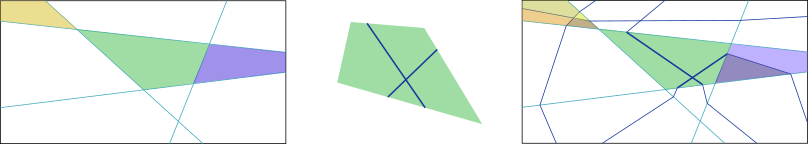
\includegraphics[width=\linewidth]{drawings/iterative_partitioning_procedure.png}
    \caption{\textbf{Left:} The bounding box represents $\mathcal{X}^{(0)}$, with each line representing the partition boundary induced by a unit of layer one. A few regions of $\Omega^{(1)}$ are highlighted, suppose that the green region corresponds to $\omega_{\boldsymbol{v}^{(1)}}^{(1)}$. \textbf{Centre:} Represents $\mathrm{aff}_{\boldsymbol{v}^{(1)}}$ with the blue lines representing the power diagram induces by the vertical projection of $\mathbf{P}^{(2)}_{\boldsymbol{v}^{(1)}}$. \textbf{Right:} Represents the power diagram $\mathrm{PD}^{(1\leftarrow 2)}_{\boldsymbol{v}^{(1)}}$ along with the other power diagrams for the other cells of $\Omega^{(1)}$. Altogether they constitute $\Omega^{(1,2)}$.}
    \label{fig:iterative_partitioning_procedure}
\end{figure}

\newthought{Layer $\ell$} recursion subdivides each cell of $\Omega^{(1,\dots,\ell-1)}$ from the previous recursion steps, forming the power diagram $$\Omega^{(1,\dots,\ell)}=\bigcup_{\boldsymbol{\nu}^{(1\leftarrow\ell-1)}}\mathrm{PD}_{\boldsymbol{\nu}^{(1\leftarrow\ell-1)}}.$$

\begin{theorem}
    Each cell $\omega_{\boldsymbol{\nu}^{(1\leftarrow\ell-1}}^{(1\leftarrow\ell-1)}\in\Omega^{(1\leftarrow\ell-1)}$ is subdivided into $\mathrm{PD}^{(1\leftarrow\ell)}_{\boldsymbol{\nu}^{(1\leftarrow\ell-1)}}$, a power diagram with domain $\omega_{\boldsymbol{\nu}^{(1\leftarrow\ell-1)}}^{(1\leftarrow\ell-1)}\in\Omega^{(1\leftarrow\ell-1)}$, centroids $$\mu_{\boldsymbol{\nu}^{(1\leftarrow\ell)}}^{(1\leftarrow\ell)}=\left(A_{\boldsymbol{\nu}^{(1\leftarrow\ell-1)}}^{(1\leftarrow\ell-1)}\right)^\top\mu_{\boldsymbol{\nu}^{(\ell)}}^{(\ell)}$$and radii $$\tau_{\boldsymbol{\nu}^{(1\leftarrow\ell)}}^{(1\leftarrow\ell)}=-\left\Vert\mu_{\boldsymbol{\nu}^{(1\leftarrow\ell)}}^{(1\leftarrow\ell)}\right\Vert^2-2\left\langle\mu_{\boldsymbol{\nu}^{(\ell)}}^{(\ell)},B_{\boldsymbol{\nu}^{(1\leftarrow\ell-1)}}^{(1\leftarrow\ell-1)}\right\rangle-2\left\langle\mathbf{1},B_{\boldsymbol{\nu}^{(\ell)}}^{(\ell)}\right\rangle,$$for every $\boldsymbol{\nu}^{(i)}\in\{1,\dots,r\}^{d^{(i)}}$ with $$B^{(1\leftarrow\ell-1)}=\sum_{\ell^\prime=1}^{\ell-1}\left(\prod_{i=\ell-1}^{\ell^\prime}A_{\boldsymbol{\nu}^{(i)}}^{(i)}\right)B_{\boldsymbol{\nu}^{\left(\ell^\prime\right)}}^{\left(\ell^\prime\right)}$$forming $\Omega^{(1\leftarrow\ell)}$.
\end{theorem}

\begin{corollary}\label{cor:deep_network_layer_convex_polytopes}
    The input space partitioning of a deep network is composed of convex polygons.
\end{corollary}

\section{Decision Boundary}

Consider the case of $r=2$ nonlinear activation operators. 

\begin{definition}
    The edges of a polytope $\mathcal{P}_i^{(\ell)}$ in a space $\mathcal{X}^{\left(\ell^\prime\right)}$, for $\ell^\prime<\ell$, are $$\mathrm{edge}_{\mathcal{X}^{\left(\ell^\prime\right)}}(i,\ell)=\left\{\mathbf{x}\in\mathcal{X}^{\left(\ell^\prime\right)}:\mathcal{E}_{i,2}^{(\ell-1)}\left(\mathbf{z}^{\left(\ell^\prime\to\ell-1\right)}(\mathbf{x})\right)=0\right\},$$where $\mathbf{z}^{\left(\ell^\prime\to\ell-1\right)}=\mathbf{z}^{(\ell-1)}\circ\dots\circ\mathbf{z}^{\left(\ell^\prime\right)}$.\footnote{Note how it is sufficient to only consider $\mathcal{E}_{i,2}^{(\ell-1)}$, due our construction Example \ref{eg:maso_activation_operators}, the piecewise continuity of the operators and the fact that $r=2$.}
\end{definition}

That is, edges are the level set curve of the unit in $\mathcal{X}^{\left(\ell^\prime\right)}$. Let $$\mathrm{Pol}^{(\ell)}(\mathbf{x})=\prod_{i=1}^{d^{(\ell)}}\left(\left[\mathbf{z}^{(\ell)}\right]_i\circ\mathbf{z}^{(\ell-1)}\circ\dots\circ\mathbf{z}^{(1)}\right)(\mathbf{x}).$$

\begin{theorem}
    The polynomial $\mathrm{Pol}^{(\ell)}$ is of order $\prod_{\ell^\prime=1}^{\ell}d^{\left(\ell^\prime\right)}$, with roots corresponding to the partitioning boundaries $$\partial\Omega^{(1\leftarrow\ell)}=\bigcup_{\ell^\prime=1}^{\ell}\bigcup_{i=1}^{d^{\left(\ell^\prime\right)}}\mathrm{edge}_{\mathcal{X}^{(0)}}\left(i,\ell^\prime\right)=\left\{\mathbf{x}\in\mathcal{X}^{(0)}:\prod_{\ell^\prime=1}^{\ell}\mathrm{Pol}^{\left(\ell^\prime\right)}(\mathbf{x})=0\right\}.$$In particular, the root order gives the dimension of the boundary.
\end{theorem}

\begin{corollary}
    The decision boundary of an $L$ layer deep network with $d^{(L)}=1$ is the edge of the last layer polytope $\mathbf{P}^{(L)}$ expressed in $\mathcal{X}^{(0)}$. Namely, $$\mathrm{DB}=\left\{\mathbf{x}\in\mathcal{X}^0:f(\mathbf{x})=0\right\}=\mathrm{edge}_{\mathcal{X}^{(0)}}(1,L)\subseteq\partial\Omega^{(1,\dots,L)}.$$
\end{corollary}

\section{References}

Results in Chapter \ref{ch:partition_geometry} from \citet{balestrieroGeometryDeepNetworks2019}.